\documentclass[a4paper,10pt]{report}

\usepackage[utf8]{inputenc}
\usepackage[english]{babel}
\usepackage[T1]{fontenc}
\usepackage{mathpazo}

\usepackage[colorlinks=true]{hyperref}
\hypersetup{urlcolor=black,linkcolor=black,citecolor=black}

\usepackage{enumerate}

\usepackage{fullpage}
\setlength{\parindent}{0pt}
\setlength{\parskip}{\medskipamount}

\usepackage{amsmath}
\usepackage{amssymb}
\usepackage{mathrsfs}
\usepackage{amsthm}
\usepackage{stmaryrd}
\usepackage{array}
\usepackage{graphicx}
\usepackage{comment}
\usepackage{pgfgantt}
\usepackage{soul} % highlight text
\usepackage{xspace} % space after new command
\usepackage{fnpct}
\usepackage{algorithm2e}
\usepackage[bottom]{footmisc}

\definecolor{bluec}{rgb}{0.7, 0.7, 1.0}
\sethlcolor{bluec} % highlight in blue

\usepackage{listings}

\newcommand{\wikidata}{\emph{Wikidata}\xspace}
\newcommand{\Wikidata}{\emph{Wikidata}\xspace}
\newcommand{\wikimedia}{\emph{Wikimedia Foundation}\xspace}
\newcommand{\Wikimedia}{\emph{Wikimedia Foundation}\xspace}
\newcommand{\wikipedia}{\emph{Wikipedia}\xspace}
\newcommand{\Wikipedia}{\emph{Wikipedia}\xspace}

\title{Projet Pensées Profondes\\\large Final report}
\author{
\includegraphics[width=0.3\textwidth]{../logo_ensl.pdf}\\[50pt]
Fundamental Computer Science Master's Degree 1\\September 2014 \--- December 2014\\[50pt]
Adviser: Eddy \textsc{Caron}\\[50pt]
\begin{minipage}{0.4\textwidth}
    \begin{flushleft} \large
        Marc \textsc{Chevalier}
        \\
        Raphaël \textsc{Charrondière}
        \\
        Quentin \textsc{Cormier}
        \\
        Tom \textsc{Cornebize}
    \end{flushleft}
\end{minipage}
\begin{minipage}{0.4\textwidth}
    \begin{flushright} \large
        Yassine \textsc{Hamoudi}
        \\
        Valentin \textsc{Lorentz}
        \\
        Thomas \textsc{Pellissier Tanon}
        \\
    \end{flushright}
\end{minipage}
}
\date{}
\vfill

\begin{document}
\maketitle

\tableofcontents

\addcontentsline{toc}{chapter}{Introduction}
\chapter*{Introduction}
    The {\em Projet Pensées Profondes} (Deep Thought Project) aims at
providing a powerful software for answering questions written in
natural language.
To accomplish this, we developped an eponymous set of tools that
accomplish different tasks and fit together thanks to a protocol
we developped.

These various tasks include data querying (using the young and open
knownledge base Wikidata), question parsing (using the
CoreNLP software written by Stanford University and machine learning),
requests routing, web user interface, and feedback reporting.

Given the young age of this projet, these pieces are only starting
to emerge with their first features and mutual communications,
so we will describe them separately in this document without
much of a general overview of the project.


\chapter{Overview}
    \begin{frame}[fragile]
    \frametitle{Architecture}
    \begin{figure}
        \resizebox{.9\linewidth}{!}{
            \newlength{\moduledistance}
\setlength{\moduledistance}{1cm}
\overfullrule=2cm
\tikzset{
    module/.style={
           rectangle,
%           rounded corners,
           draw=mDarkTeal, very thick,
           minimum width=3cm,
           minimum height = 0.7cm,
           node distance = 1.5cm,
           inner sep=2pt,
           text centered,
           },
}

\tikzset{
    core/.style={
           circle,
           draw=mDarkTeal, very thick,
           minimum width=2cm,
           inner sep=2pt,
           text centered,
           },
}

\tikzset{
    arrow/.style={
           ->,
           draw=mDarkTeal, very thick,
    }
}

\tikzset{
    darrow/.style={
           <->,
           draw=mDarkTeal, very thick,
    }
}

\begin{tikzpicture}[->,>=stealth']
    \node[core] (core) {
        Core
    };
    \node[module,
          right of=core,
          right=\moduledistance,
          ] (grammatical) {
          Grammatical
    };
    \node[module,
          below of=grammatical,
          ] (standalone) {
        \begin{tabular}{c}
        Machine Learning\\Standalone
        \end{tabular}
    };
    \node[module,
          above of=grammatical,
          ] (reformulation) {
        \begin{tabular}{c}
        Machine Learning\\Reformulation
        \end{tabular}
    };
    \node[module,
          left of=core,
          left=\moduledistance,
          ] (wikidata) {
        Wikidata
    };
    \node[module,
          above of=wikidata,
          ] (cas) {
        Computer Algebra
    };
    \node[module,
          below of=wikidata,
          ] (spellchecker) {
        Spell-checker
    };
    \node[module,
          above of=core,
          above=1cm,
          ] (webui) {
        \begin{tabular}{c}
        Web User\\
        Interface
        \end{tabular}
    };
    \node[module,
          above of=reformulation,
%          right=\moduledistance,
          ] (logging) {
        Logging backend
    };
    \draw[mLightBrown,thick] ($(reformulation.north west)+(-0.3,0.3)$)  rectangle node[yshift=-2.5cm,below] {Question Parsing} ($(standalone.south east)+(0.3,-0.3)$);
    \draw[mLightBrown,thick] ($(cas.north west)+(-0.3,0.3)$)  rectangle node[yshift=-2.5cm,below] {Other modules} ($(spellchecker.south east)+(0.3,-0.3)$);

    \draw [darrow] (core)          -- node{} (cas.south east);
    \draw [darrow] (core)          -- node{} (wikidata.east);
    \draw [darrow] (core)          -- node{} (spellchecker.north east);
    \draw [darrow] (core)          -- node{} (reformulation.south west);
    \draw [darrow] (core)          -- node{} (grammatical.west);
    \draw [darrow] (core)          -- node{} (standalone.north west);
    \draw [darrow] (core)          -- node{} (webui.south);
    \draw [darrow] (webui)         -- node{} (logging.west);
    \draw [arrow]  (logging)       -- node{} (reformulation.north);
    \draw [arrow]  (grammatical)   -- node{} (reformulation.south);

\end{tikzpicture}

        }
    \end{figure}
\end{frame}

\begin{frame}[fragile]
    \frametitle{Datamodel}
    How to represent formally a question asked in natural language?

    \alert{Tree} structure.
\end{frame}
\begin{frame}[fragile]
    \frametitle{Datamodel \--- Leaves: resources}
        \begin{itemize}
            \item Strings: "Isaac \textsc{Newton}"
            \item Dates: 25 December 1642
            \item Geographic coordinates: 47° 30' 18'' N ; 9° 44' 57'' E
            \item \ldots
        \end{itemize}
\end{frame}
\begin{frame}[fragile]
    \frametitle{Datamodel \--- Nodes: operations}
        \begin{itemize}
            \item Full \alert{triples}: (Isaac \textsc{Newton}, birth date, 25 December 1642 (Julian)) $\rightarrow$ true
            \item Missing: (?, birth date, 25 December 1642 (Julian)) $\rightarrow$ [Isaac \textsc{Newton}]
            \item Union, Intersection, Difference, \ldots
            \item And, Or, Not
            \item Exists
            \item Sort, First, Last
        \end{itemize}
\end{frame}

\begin{frame}[fragile]
    \frametitle{Datamodel \--- Examples}
    \begin{itemize}
        \only<1>{
        \item \alert{"Is Brussels the capital of Belgium and the European Union?"}
          \begin{center}
            \begin{figure}
          \resizebox{\linewidth}{!}{
            \begin{tikzpicture}
              \node (0) at (10,8.5) {$\bigwedge$};
              \node (1) at (7,7) {$\triple$};
              \node (11) at (5,5.5) {Brussels};
              \node (12) at (7,5.5) {capital};
              \node (13) at (9,5.5) {Belgium};
              
              \node (2) at (13,7) {$\triple$};
              \node (21) at (11,5.5) {Brussels};
              \node (22) at (13,5.5) {capital};
              \node (23) at (15,5.5) {European Union};

              \node (9) at (14,1) {}; % utilisé pour forcer le positionnement de la figure globale

              \draw[->, >=latex] (0) edge node[sloped, anchor=center, above] {} (1);
              \draw[->, >=latex] (1) edge node[sloped, anchor=center, above] {\scriptsize{subj.}} (11);
              \draw[->, >=latex] (1) edge node[sloped, anchor=center, above] {\scriptsize{pred.}} (12);
              \draw[->, >=latex] (1) edge node[sloped, anchor=center, above] {\scriptsize{obj.}} (13);
              \draw[->, >=latex] (0) edge node[sloped, anchor=center, above] {} (2);
              \draw[->, >=latex] (2) edge node[sloped, anchor=center, above] {\scriptsize{subj.}} (21);
              \draw[->, >=latex] (2) edge node[sloped, anchor=center, above] {\scriptsize{pred.}} (22);
              \draw[->, >=latex] (2) edge node[sloped, anchor=center, above] {\scriptsize{obj.}} (23);
             \end{tikzpicture}
            }
            \end{figure}

          \end{center}}
            
        \only<2>{
        \item \alert{"Who is the mayor of the capital of Kreis Bergstraße?"}
          \begin{center}
            \begin{forest}
              [\texttt{Triple}[\texttt{Triple}[Kreis Bergstraße][capital][?]][mayor][?]]
            \end{forest}
          \end{center}}
            
        \only<3>{
          \item \alert{"What is the birth date of the first president of Germany?"}
          \begin{center}
            \begin{forest}
              [\texttt{Triple}[\texttt{First}[\texttt{Sort}[\texttt{Triple}[Germany][president][?]][mandate begin date]]][birth date][?]]
            \end{forest}
          \end{center}}

        \only<4>{
          \item \alert{"Is there a medical treatment for Ebola?"}
            \begin{center}
              \begin{forest}
                [\texttt{Exists}[\texttt{Triple}[Ebola][medical treatment][?]]]
              \end{forest}
            \end{center}}

        \only<5>{
          \item \alert{"Who are the children of François \textsc{Mitterrand} and Anne \textsc{Pingeot}?"}
            \begin{center}
              \begin{forest}
                [$\bigcap$[\texttt{Triple}[François \textsc{Mitterrand}][child][?]][\texttt{Triple}[Anne \textsc{Pingeot}][child][?]]]
              \end{forest}
            \end{center}}


    \end{itemize}
\end{frame}


\chapter{State of the art}
    Our project is about \textit{Question Answering}, a field of research included in \textit{Natural Language Processing} (NLP) theory. NLP mixes linguistic and computer science and is made of all kinds of automated techniques that have to deal with natural languages, such as French or English. For instance, automatic translation or text summarization are also parts of NLP.

In Natural Language Processing, sentences are often represented in a condensed and normalized form called \textit{(subject, predicate, object) triple representation}. For example, the phrase ``Fleming discovered penicillin.'' will be represented by the triple (penicillin, discoverer, Fleming). Two triples can be associated to ``The president was born in 1950 and died in 2000.'': (president, birth date, 1950) and (president, death date, 2000). This representation has been formalized into the \textit{Resource Description Framework} (RDF) model\footnote{\url{http://www.w3.org/TR/rdf11-concepts/}}. It consists of a general framework used to describe any Internet resource by sets of triples. One of our main goals is to parse questions to get their triples representation.

Many algorithms have been developed since fifty years with the objective of understanding the syntax and the semantic of sentences in order to extract (subject, predicate, object) triples. Two popular graph representations are widely used:
\begin{itemize}
 \item parse structure tree. It tries to split the sentence according to its grammatical structure. Figure .. presents the parse structure tree of \textit{...}. For instance, .. means ...
 \item dependency tree. It reflects the grammatical relationships between words. The dependency tree of \textit{..} is  . The relation .. means for example that .. is ...
\end{itemize}
Existing libraries, such as \textit{NLTK}\footnote{\url{http://www.nltk.org/}} or \textit{StanfordParser}\footnote{\url{http://nlp.stanford.edu/software/lex-parser.shtml}} provide powerful tools to extract such representations.

We did not find a lot of detailed articles exposing procedures to get triples from the grammatical structure. For instance \cite{parsetree} tries to perform the extraction using the parse structure tree. However we believe the dependency tree could be more appropriate since it is more focused on the relations between the words than their roles in the sentence. Part \ref{gramap} presents an algorithm we have designed using the dependency tree representation.

We have also observed a growing use of machine learning techniques in NLP that try to automatically learn triples extraction rules instead of building intermediate grammatical representations. We will use such machine learning algorithms in parts \ref{mlreformulation} and \ref{mlwindow}.

Finally, some existing tools are very close to our goal\footnote{\url{http://quepy.machinalis.com/}}\textsuperscript{,}\footnote{\url{http://www.ifi.uzh.ch/ddis/research/talking.html}}. They allow us to have a clear idea of the state of the art, and what performances in question answering we can expect.

\chapter{Data model and communication}
    We describe the choices we did about representation of the data and communication between modules.

\section{Data model}
\label{rdf}

First, we present the data model. All normalized structures of the PPP are JSON-serializable, i.e. they are trees made of instances of the following types:
\begin{itemize}
    \item \texttt{Object}
    \item \texttt{List}
    \item \texttt{String}
    \item \texttt{Number}
    \item \texttt{Boolean}
    \item \texttt{Null}
\end{itemize}

We chose to represent all normalized data as trees. To represent sentences, we have 4 kinds of nodes.

\begin{itemize}
    \item \texttt{sentence}: a question in natural language like "Who is George Washington?".
    \item \texttt{resource}: a leaf containing any kind of data (string, integer\ldots).
    \item \texttt{missing}: a leaf which marks missing values.
    \item \texttt{triple}: a 3-ary node:
        \begin{itemize}
            \item \texttt{subject}: what the triple refers to
            \item \texttt{predicate}: denotes the relationship between the subject and the
  object
            \item \texttt{object}: what property of the subject the triple refers to
        \end{itemize}         
\end{itemize}

For example, the work of the question parsing module is to transform 
\begin{verbatim}
{
    "type": "sentence", 
    "value": "Who is George Washington?"
}
\end{verbatim}
into 
\begin{verbatim}
{
    "type":
        "triple",
    "subject":{
        "type": "resource",
        "value": "George Washington"
    },
    "predicate":{
        "type": "resource",
        "value": "identity"
    },
    "object":{
        "type": "missing"
    }
}
\end{verbatim}

This structure has been chosen for its good adaptability. For instance, we can add other kind of nodes such as intersection, union, node for yes/no questions (triples without missing son), boolean operations etc..

As every tree which has ordered children, we can represent them as a string. We chose the order of the different fields in the implementation: subject, predicate, object.

To print these tree in the user interface, we do not print explicitly the \texttt{resource} nodes. A \texttt{missing} node is symbolized by a "\texttt{?}" possibly followed by an id (an integer).

For instance, the previous tree will be represented by the string:
\begin{verbatim}
(George Washington, identity, ?)
\end{verbatim}

\section{Communication}

Modules communicate with the core via HTTP requests.

The core sends them a JSON object, and they return another one.

The basic idea is that the core iterates requests to modules, which return a simplified tree, until the former gets a complete response.

During these exchanges, we keep a trace of the different steps between the original request and the current tree. The structure of a trace is a list of such trace items:
\begin{verbatim}
{
    "module":
        "<name of the module>", 
    "tree":{
        <answer tree>
    },
    "measures":{
        "relevance": <relevance of the answer>,
        "accuracy": <accuracy of the answer>
    }
}
\end{verbatim}

The measure field contains two values: relevance and accuracy.

\begin{itemize}
    \item \texttt{accuracy} is a self-rating of how much the module may have correctly understood (ie. not misinterpreted) the request/question. It is a float between 0 and 1.
    \item \texttt{relevance} is a self-rating of how much the tree has been improved (i.e. made its way from a question to an useful answer). A positive float (not necessarily greater that 1; another module might use it to provide a much better answer).
\end{itemize}

This form allows each module to access to the previous results, particularly to the user's request. The objects for request and response contains few more information such that the language used.

The data model have been implemented in a nice set of objects in both \href{http://github.com/ProjetPP/PPP-datamodel-Python}{Python} and \href{http://github.com/ProjetPP/PPP-datamodel-PHP}{PHP} in order to help the write of modules.

We could define a linear representation for the trace, using the representation of the datamodel, but it is not relevant. Indeed, this information will never be printed on the user interface.

\begin{figure}[!ht]
% https://docs.google.com/drawings/d/1toUH24GqwtpvKV7S5gje6GBxfa13R3mxgm8WlAFc_0g/edit?usp=sharing
  \centering
    \label{struct}
    \caption{Architecture of the PPP}
    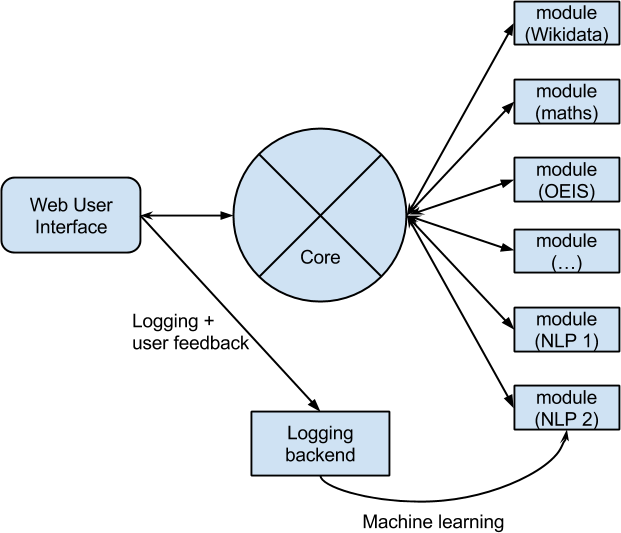
\includegraphics[width=0.5\textwidth]{../ppp_structure.png}
\end{figure}


\chapter{Core}
    \section{Communications}

As its name suggests, the core is the central point of the PPP. It is
connected to all other components — user interfaces and modules — through
the protocol defined above.

The core communicates with the user interfaces and the modules {\em via} HTTP:
each time the core receives a requests from an interface, it forwards it
to modules, using a configurable list of URL where to reach modules.

An example configuration is the one we use on the production server:

\begin{verbatim}
{
    "debug": false,
    "modules": [
        {
            "name": "nlp_classical",
            "url": "http://localhost:9000/nlp_classical/",
            "coefficient": 1
        },
        {
            "name": "flower",
            "url": "http://localhost:9000/flower/",
            "coefficient": 1
        },
        {
            "name": "wikidata",
            "url": "http://wikidata.ppp.pony.ovh/",
            "coefficient": 1
        }
    ]
}
\end{verbatim}

The current state is the the Core is successfully able with all modules
that have been written: the Wikidata module, an example Python module
(which answers the question  “Who are you?”), and the Natural Language
Processing module.

\section{Routing}

Besides from communicating with other pieces of the PPP, the Core will
also route requests in such a way the power of the modules can be
combined to give something greater.

For instance, when a user will input a question like “Who is the first
president of the United States?”, the Core will send the question to
all modules and get a parsed tree from the Natural Language Processing
module. Then, it will forward this answer to all other modules, which the
Wikidata module will be able to answer.

This part is not implemented, but will be next step in the implementation
of the Core.


\chapter{User interface}
    \chapter{User Interface}

We decided to implement first only a web user interface. This interface
is only composed of one web-page developed in HTML 5 with some
pieces of JavaScript and CSS. We have taken care of having an
interface that fit nice on both huge screens of desktop computers
and small screens of phones.

TODO: screenshot 

It is composed of only one huge text input with a button to submit
the query and an other one to get a random question. The text area
allows both the input of questions in English or directly of triple using
an easy notation like \texttt{(Douglas Adam, birth date,?)} to find the
birth date of Douglas Adam. A small parser written in JavaScript convert
this easy to use notation into the standard format.

In order to build this interface we have relied on some famous libraries 
ike \href{http://jquery.com/}{jQuery} and \href{http://getbootstrap.com/}{Bootstrap}.

\section{Logging}

We decided to log all requests made to the PPP to improve our algorithms,
and particularily to feed the results to Natural Language Processing
modules that use Machine Learning.
We may also use it to improve the way the Core routes/sorts answers
from the different modules, either manually or with some basic
Machine Learning.

The main idea is to log user feedback in addition to the requests
themselves: after showing the user the way we interpreted their
question alongside the answer to their request, we provide them a
way to give us feedback.
What we call feedback is actually a thumb up / thumb down pair of
buttons, and, if the latter is pressed, a way to correct the requests
parsing result so it can be fed to the Machine Learning algorithms.

Since Machine Learning algorithms are not ready yet, we did not focus
on this feature of the user interface and thus it is not implemented;
so far we only started implemented a backend that stores data
(gathered via the user interface) to a SQLite database.


\chapter{Question parsing}
    
The goal of this module is to transform questions into trees of triples, as described in section \ref{rdf}, which can be handled by backend modules.

The difficulty of this task can be illustrated on the following example: 
\begin{center}
 \textit{What is the birth date of the president of the United States?}
\end{center}

A first possible tree is: \hl{(?,birth date, president of the United States)}. However, this tree is difficult to handle by databases-querying modules. Indeed, the ``president of the United States'' occurence in a database probably does not contain the birth date of the current president. 

On the other hand, the following tree is much more easy to process : \hl{(?,birth date, (?,president of, United States))}. In this case, the president of United States is identified (\hl{Barack Obama}), the triple becomes \hl{(?,birth date, Barack Obama)}, and finally the answer can be found easily in ``Barack Obama'' occurence.

Our goal is to product simplified and well structured trees, without losing relevant informations of the original question. We are developing three different approaches to tackle this problem. The first tries to analyze the grammatical structure of questions, the two other ones are based on machine learning.
    \section{Grammatical approach}

Trees of triples can be produced after analysing the grammatical structure of sentences. First, we  present the tool we use to extract grammatical dependencies. Then, we expose chronologically our algorithm to product triples from grammatical structure.

We will detail throughout this section our algorithm on the example:
\begin{center}
 \textit{What is the birth date of the president of the United States?}
\end{center}

%########################################################################################%

\subsection{\Stanford}

The \Stanford library \footnote{\url{http://nlp.stanford.edu/software/corenlp.shtml}} is a tool developed by the \emph{Stanford Natural Language Processing group}, composed of linguists and computer scientists. This software is well-documented and considered as a ``state of the art'' tool. Moreover, it includes very efficient grammatical parsers.

Since this library is written in Java, and our module in Python, we use a Python wrapper\footnote{\url{https://bitbucket.org/ProgVal/corenlp-python/overview}} we first patched to support Python 3 and some features the wrapper did not implement.

We use \CoreNLP mostly to get grammatical dependency trees from input questions. It consists in trees which nodes are the words of the sentence, and edges reflect the grammatical relations between words.

Figure \ref{tree_one} provides an overview of such a tree on our question example \emph{What is the birth date of the president of the United States?}. For instance, the edge:
  \[\texttt{president}\xrightarrow{\texttt{det}}\texttt{the}\]
means that \emph{the} is a determiner for \emph{president}.

\begin{figure}
  \centering
  \caption{Dependency tree}
  \label{tree_one}
    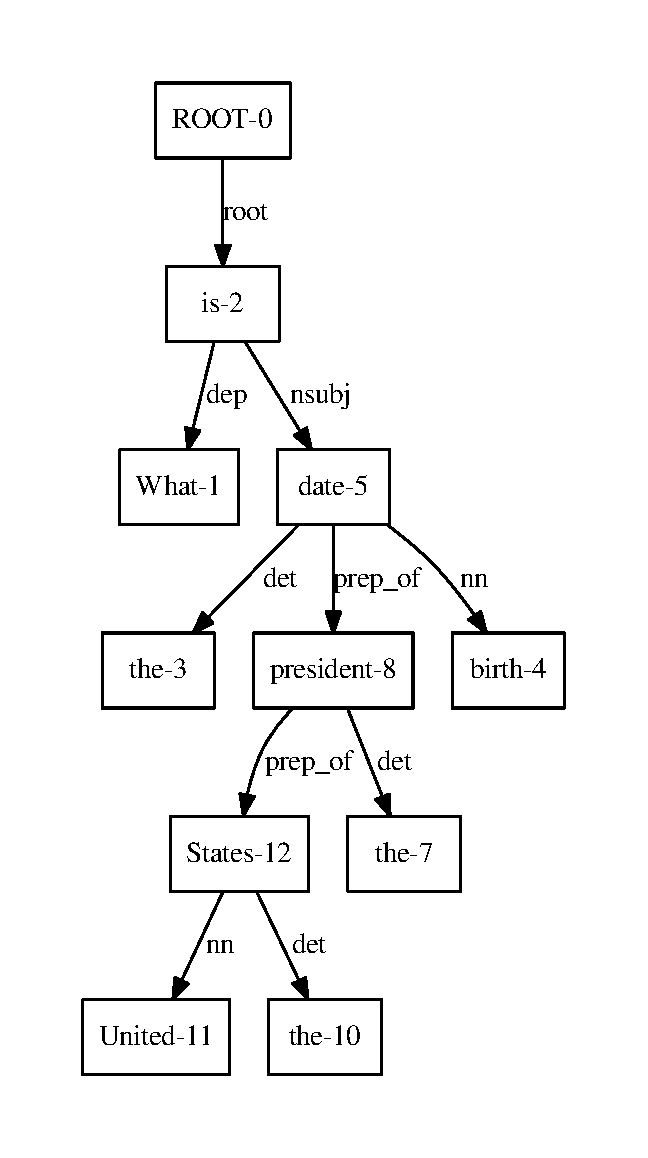
\includegraphics[scale=0.6]{../examples_NLP_grammatical/tree1.pdf}
\end{figure}

Some nodes of this tree are also endowed with tags. For example, \emph{United} and \emph{States} have the tag \emph{location}.

The Stanford typed dependencies manual (\cite{stanfordDep}) provides a full list and description of possible grammatical dependencies.

%########################################################################################%

\subsection{Preprocessing}

The preprocessing consists in a sequence of operations executed on the tree outputs by the \Stanford library. The aim is to simplify it, by merging the nodes which should belong together.

The current version of the module performs two sorts of merges:
\begin{itemize}
    \item \textbf{Merge quotation nodes.} This operation merges all the nodes which are in a same quotation (delimited by quotation marks). It also adds the words
    of the quotation which were deleted by the \Stanford library (e.g. \emph{in}, \emph{of}\dots). The final result is a node, containing the
    exact quotation, and placed at the appropriate position in the tree.
    
    \item \textbf{Merge named entities.} The \Stanford library performs a \emph{named entities recognition} (NER), which provides informative 
    tags in some nodes. For instance, \emph{United} and \emph{States} are tagged \emph{LOCATION} (see figure \ref{tree_two}). In the preprocessing step, we merge all neighbour nodes with a same NER tag. In our example, we merge the two nodes \emph{United States} into one single node.
\end{itemize}

The preprocessing also identifies the question word (Who, What, Where...) and removes it from the dependency tree.

Preprocessing is illustrated on figure \ref{tree_two}. The question word is \textit{What}.

\begin{figure}
  \centering
  \caption{Dependency tree preprocessed}
  \label{tree_two}
    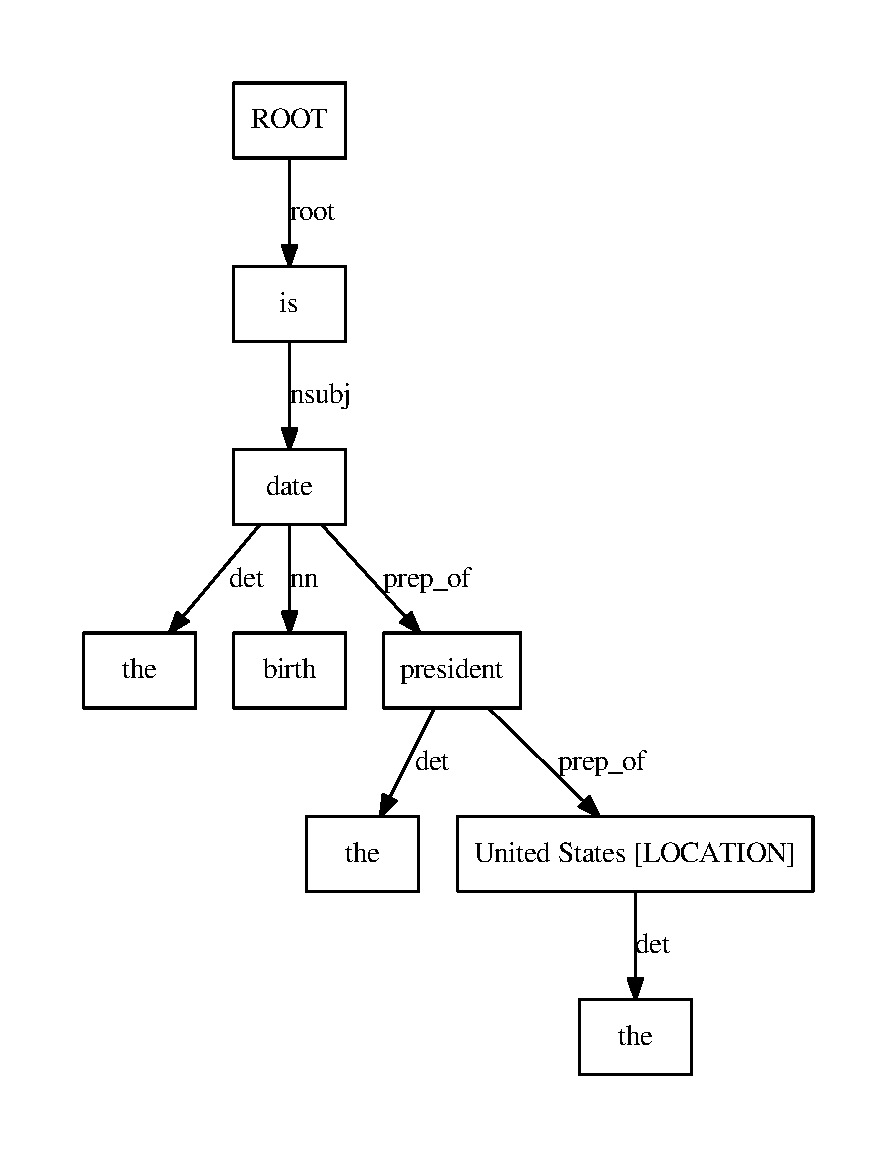
\includegraphics[scale=0.6]{../examples_NLP_grammatical/tree2.pdf}
\end{figure}

%########################################################################################%

\subsection{Grammatical dependencies analysis}

The grammatical tree is simplified by applying one of the following rules to each edge:
\begin{itemize}
 \item remove the edge and its endpoint node. For instance, a \textit{dep} relation, such as \textit{the} in our example, is often removed.
 \item merge the two nodes of the edge. Merge operations try to gather words of a same expression (e.g. phrasal verbs) that have not been merged during preprocessing.
 \item tag the edge with a ``triple production rule''.
\end{itemize}

The third operation is the most important. Dependencies relations are replaced by a restricted set of tags that will enable us to product a triples tree thereafter.

On our example, the edge:
\[\texttt{birth}\xrightarrow{\texttt{nn}}\texttt{date}\]

is merged into a single node : \textit{birth date}.

One of the triples production rules tag is : 

\[\texttt{is}\xrightarrow{\texttt{t1}}\texttt{birth date}\]

The simplified tree of our example is illustrated on figure \ref{tree_three}.

\begin{figure}
  \centering
  \caption{Dependency tree simplified}
  \label{tree_three}
    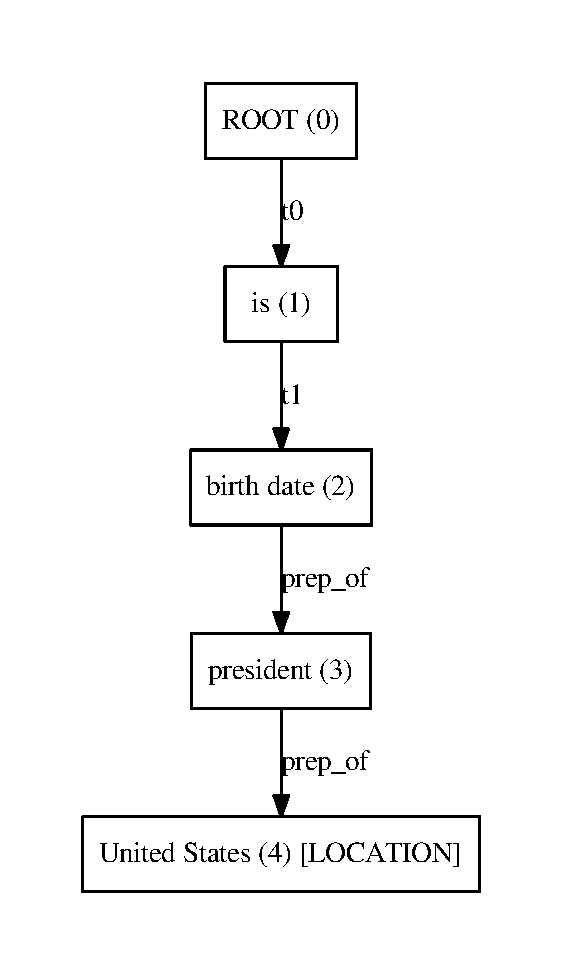
\includegraphics[scale=0.6]{../examples_NLP_grammatical/tree3.pdf}
\end{figure}

%########################################################################################%

\subsection{Triples production}

The triples production is the final step. It outputs the triples tree.

First, we assign a number to each remaining node. The root of the tree has always number \textit{0}. We have directly print these numbers on figure \ref{tree_three}.

Then, we associate to each subtree of root's number \textit{x} an unknown denoted \textit{?x} that identifies the information the subtree refers to. On our example, the subtree of root \textit{president} (number \textit{3}) represents the name of the president of the United States. This unknown is denoted \textit{?3}.

Unknowns are linked together into triples thanks to the triples production rules tagged previously. For instance, an  edge tagged \textbf{t2}:

\[\texttt{a}\xrightarrow{\texttt{t2}}\texttt{b}\]

products the triples \hl{(?a,a,?b)}, or \hl{(?a,a,b)} if b is a leaf (a and b are replaced by the words of the node they refer to).

The tag \textbf{t1} directly linked two unknowns \hl{?a = ?b}, instead of producing a triple.

The tag \textbf{t0} products nothing.

We obtain the following result on our example:

\begin{center}
 ?1 = ?2 ~\\
 (?2 , birth date of , ?3) ~\\
 (?3 , president of , United States)
\end{center}

Then, we link \textit{?0} to \textit{?1}, depending on the question word of the question. Here we have (question word \textit{What}):
\begin{center}
 (?1,definition,?0)
\end{center}

The four previous rules are simplified in a set a triples:

\begin{center}
 (?1,definition,?0) ~\\
 (?1 , birth date of , ?3) ~\\
 (?3 , president of , United States)
\end{center}

Find an answer to the question is equivalent to build a model of the conjunctive formula: \textbf{(?1 , definition , ?0)$\wedge$(?1 , birth date of , ?3)$\wedge$(?3 , president of , United States)} and outputs the value of \textit{?0}.

The triples tree is obtained by replacing each unknown \textit{?x} by a triple containing \textit{?x} \textit{and not} \textit{?0}. The final result, taken from the PPP website, is printed on figure \ref{tree_four}. Figure \ref{triple_tree} contains the formal representation of the triples tree of our example.

\begin{figure}[!h]
  \centering
  \caption{Triples tree}
  \label{tree_four}
    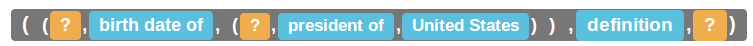
\includegraphics[scale=0.5]{../examples_NLP_grammatical/final_result.png}
\end{figure}

Backend modules (such as Wikidata module) will have to fill intermediate unknowns : \hl{((August 4 1961,birth date of, (Barack Obama, president of, United States)), definition, ?)} and finally provide the final answer that replaced \textit{?} (for example: a description of the August 4 1961 date).


%########################################################################################%

\subsection{Future work}

\subsubsection{Grammatical rules analysis}

Our analysis of grammatical rules, in order to product triples, is very basic. Currently, we only have about 5 rules. Although it is good enough to handle a lot of questions, we are not able to process conjunctions for example (e.g. \textit{``Who wrote "Lucy in the Sky with Diamonds" and "Let It Be"?''}).

\subsubsection{Preprocessing merging}

There remains nodes which should stay together but are not merged by our module, for instance \emph{prime minister} or \emph{state of the art}. Recognizing such words is called \emph{Multiword Expressions Processing}. This task is a whole part of Natural Language Processing theory. 

We have several tracks to improve merging. Existing algorithms or softwares need to be tested. We could also use multiword expressions dictionaries.

\subsubsection{Question type analysis}

The current algorithm attaches great importance to the type of the input question. Sentences starting by a question word (Who, Where, How ...) are better processed than Yes/No questions for instance.

\subsubsection{Triples tree improvement}

The triples tree will be improved to take into account new types of nodes, adapted to databases queries. For example, a node could be tagged ``FIRST'' to pick the first occurrence of a list of answers (e.g. \hl{FIRST(?,presidents of, United States)}).

    \section{Reformulation : a learning approach }

Efficiency of neural network nowadays can be very good. An approach based on network is also used here. But, the aim is not to learn answering question, there are two reasons for that: first the knowledge changes over time, e.g. the president name depends of the date, then something simple is wished, the learning process should also be continuous. In the second case, learning the answer implies to know proper Names which increase the size of the dictionary, that means the learning time. The module presented here try to reformulate a question. In fact it try to translate the question for the wikidata module.

\subsection{How it works}

There is a output of the grammatical module which builds a triple representation of the question. All work is done on this representation. The assumption ``all useful information is keep in this form''  is also necessary. The module has also a dictionary. There are four step to do. First a pretreatment replace proper names and numbers with tags, such that all word of the triple are in the dictionary, then the request is projected in the math space of request. Two last step reveres the two first, but the reverse projection should produce a better request, which mean the final request is adapted for the Wikidata module.

\subsubsection{Mathematical spaces}

The mathematical space of request $\mathcal{R}$ is simply the subset of the $\mathbb{R}$ vector space of dimension 50, were all vector have an euclidean norm of 1.
A triple is formed of a subject request, a predicate and an object request, it is also natural to consider the triple over $\mathcal{R}$, and matching will always follow the order subject, predicate, object.
Let us call vector the elements of $\mathcal{R}$.
The choice of a 50-dimension can be modified if necessary, but taking a higher dimension could slow the learning process, and with a lower space we could lost some expression power, which may lead to very poor results.

%To unify everything As we works with requests, we consider everything is a request, even a word.

%There are 2 generic spaces: the one of words which is a vector space of dimension 50 and the space of request which is the space of word triples. The first word of a triple represents the subject, the second represents the predicate and the last the object.
%To distinguish words which are vectors and words with letters, we will add the adjective English to the seconds.

\subsubsection{Dictionary}

The dictionary defines matching between English words and vectors triple, which is the base of the process. We use triple because a word could have different meaning depending on his nature, so predicate vector for a word is not the same as subject vector which is not the same as object vector. We will denote m.s vector-subject of word m, m.p and m.o for predicate and object.

\subsubsection{Pre- and post-treatment and treatment}

We evoke some reasons not to handle proper name directly (the dictionary size would increase and names could changes), there is another arguments: there is an arbitrary number of proper names, because you can invent some new names every time. That is why they are replace in a request by a tag NAMEi, $i\in{1,2,3}$. It allows us to have three different names in a question, and that is sufficient. The same happens for numbers. Tag UNKNOWN finally represents the ``holes'' in the request tree. At the end, after the treatment we replace tags with corresponding real names or numbers in the final tree.

Recognizing a number is not hard, in fact it is just checking it the characters sequence looks like numbers optionally followed by a dot and numbers. If the sequence is not a number or a ``hole'' and is not in the dictionary, the module treat it as a proper name.

\subsubsection{Project form a request to a vector}

The model allow an arbitrary request form, it mean we have a three with an unknown depth, and to keep the complete question information we should handle it so. But the request are triple, so it is easy to transform. First with the dictionary all word are replaced with vectors, of course we take the vector corresponding to the function of the word in the tree. Then we have to ascend the whole three to compute the root value.

Let define a matrix compact which take a triple of vector and merge them in one vector, here merging in not a intuitive operation, in fact we don't known how to merge this triple, that is why all coefficients of the matrix are unknown. To compute what we call a vector, output should be normalized.

Now by applying this operation bottom-up in the tree. Main idea is each node value represent the subtree request.


\subsubsection{Reconstruct a request from a vector}

This operation is quite symmetrical of the projection, with a matrix uncompact we can the same way obtain a vector triple from a vector, and recursively an tree appears. But the question is how to known if we should reapply the function uncompact or leave the vector as a leaf? First say in a triple predicate is never a tree, then object and subject will be let as leaf if a known word is near enough. Finally each node is replace with the nearest corresponding word of the dictionary, that mean for example for a vector in middle of a triple which is also a predicate take word with nearest predicates' vector.

Defining near enough is difficult. To avoid infinite loop we will take depth of nodes into account. We must take $\delta>0$ a precision factor and $g$ a growth factor. If $d$ is depth of node $n$, near enough means distance is bounded by $\delta*g^d$ with regard of euclidean norm.  

The algorithm is also :



\begin{algorithm}[H]
    \DontPrintSemicolon  % Some LaTeX compilers require you to use \dontprintsemicolon instead
    \KwIn{$\delta>0$ et $a\in A$}
    \KwOut{request tree}
    $(s,p,o) \gets \text{uncompact}(a)$\;
    Find m s.t. $\N{m.s-s}<\delta$ is minimal \;
    \lIf{m exists}{
        $s \gets m.s$
    }
    \lElse{
        $s \gets C(\delta,s)$
    } 
    Find m s.t. $\N{m.o-o}<\delta$ is minimal \;
    \lIf{m exists}{
        $o \gets m.o$
    }
    \lElse{
        $o \gets C(\delta,o)$
    } 
    $p \gets \underset{m}{\text{argmin}}.r (\N{m.r-m.p})$\;
    \Return{$(s,r,o)$}\;
    \caption{From vector to tree}
\end{algorithm}



\subsubsection{Remarks}

Matrix compact and uncompact are not bijective after restraining the request space to existent requests. Applying uncompact then compact should give the identity, with of course an error margin, but when compacting then uncompacting we only have to find an equivalent request, i.e. with the same meaning but with another formulation. If it were not the case it would produce exactly the same out as the input, that would be useless.

\section{Learning}

Training the model can not be done easily with a classical back-propagation because we have no idea what is the best triple for a question. The solution is also to try to change a little the matrix, and see what changes improve the best the quality of result, it is however very bad in cost. 

Now to compute the quality of result, i.e. the score  of the module we use a semantic distance: it's a norm depending of the mean of words. To be simple we base it of the relation graph ``instance of'' of Wikidata assuming it is a directed acyclic graph. We compute the nearest common ancestor and we add the distance between this node and the two word  nodes.

\subsection{Implementation}

The module is written in C++, with threads to speed up the matrix multiplication. To interface it with the others, it is build as a shared library with python library. The dictionary has been generated using the clex \footnote{\url{https://github.com/Attempto/Clex}}. 

\subsection{Future work}

Learning process is not made yet. As latency with Wikidata is very high (several seconds) we have to download Wikidata and run it in local.

Then we could think of different manners to train the model.

%Finding a way to learn everything with first or second approach is the most important, as the first answering module in functional, learning is possible. Then, learning and computation speed-up will be important, the search for nearest neighbor is long, maybe it is linear, but with near 100 000 words and high dimension it becomes consequent, use of heuristics could be a good idea, for example there exists distance sensitive hash. Kd-trees allow a search in log-time (with precomputation) ; but with dimension 50, the constant factor $2^{50}$ is too large. 


    \section{Machine Learning: Window approach}

The goal of this module is to make an alternative to the grammatical approach, to product triples from English sentences.

We used machine learning algorithms in order to produce triples from scratch, without any grammatical library like \Stanford.


Motivations come from three points:
\begin{itemize}
\item Because triples are linked to the semantic of the sentence, and not directly from the grammar, we could expect that avoid grammatical tools can be a good idea.
\item It has been shown that a machine learning approach can produce, for a large panel of different NLP problems, very good solutions, closed to \textit{state of the art} algorithms \cite{collobert}.
\item Grammatical approaches fail on keyword sentences, like "Barack Obama birth date" because this kind of sentences does not respect the syntax of English.
\end{itemize}

This work is mainly based on the paper "Natural Language Processing (almost) from Scratch" \cite{collobert}.

Due to the restricted amount of time, we emphasis on keywords questions (keywords questions can't be analysis with grammatical tools) and we limit ourself to a restricted version of the data model:
\begin{itemize}
\item Only one level of depth: for example the sentence "What is the birth date of the president of the United States?" will be converted to the triple: \hl{(president of the United States, birth date, ?)}. 
\item We do not support \textit{types}, and connectors like \textit{first}, \textit{sort}...
\end{itemize}
We used a look-up table and a window approach neural network as explain below. The complete package\footnote{\url{https://github.com/ProjetPP/PPP-NLP-ML-standalone/}} was written in Python 3. We use the scikit-learn library, numpy and nltk as external tool.

Our algorithm can be described with three components: the look up table, the window approach, and the classifier.

\subsubsection{Look-up table}

The look-up table is a dictionary that associates to each word $w$ a vector $V_w \in \mathbb{R}^n$, where n is the number of parameters used to encode a word (we used $n=25$).
If two English words $w_1$ and $w_2$ are synonymous, then $||w_1-w_2||_2$ is small.

The construction of the look-up table is described in \cite{collobert} and used unsupervised machine learning techniques.
We used the pre-computed look-up table found here: \url{http://metaoptimize.com/projects/wordreprs/}

We also add one parameter to know if the word starts with a capitalize character or not. Finally, words are embedded in vectors of dimension 26. 

\subsubsection{Window approach}

We used a window (as explain in \cite{collobert}) that focuses on one word to classify. For example, if the sentence is "What is the birth date of the president of France?", and the word to classify is "date", for a window size of 7, the window is: "is the birth \textbf{date} of the president".


We used this window because classifier algorithms usually work with a fixed number of input parameters. 

The window size is a meta parameter to choose. This window has to be large enough that we can decide in the context of the window in which category a word is. We used a window of size 9.

\subsubsection{The classifier}

If the question is "What is the birth date of the president of France?", and the focus of the window approach is on the word \textbf{date}, then the goal is to classify the word \textbf{date} into one of these four categories: \textit{subject}, \textit{predicate}, \textit{object}, \textit{to forget}.

The classification of each word of the sentence into these four categories finally give us the desired triple.

The principle of the complete algorithm can be summarize in the figure ~\ref{sandalone:model}.

\begin{figure}[!ht]
  \centering
  \caption{The architecture of the algorithm, as described in \cite{collobert}}
  \label{sandalone:model}
    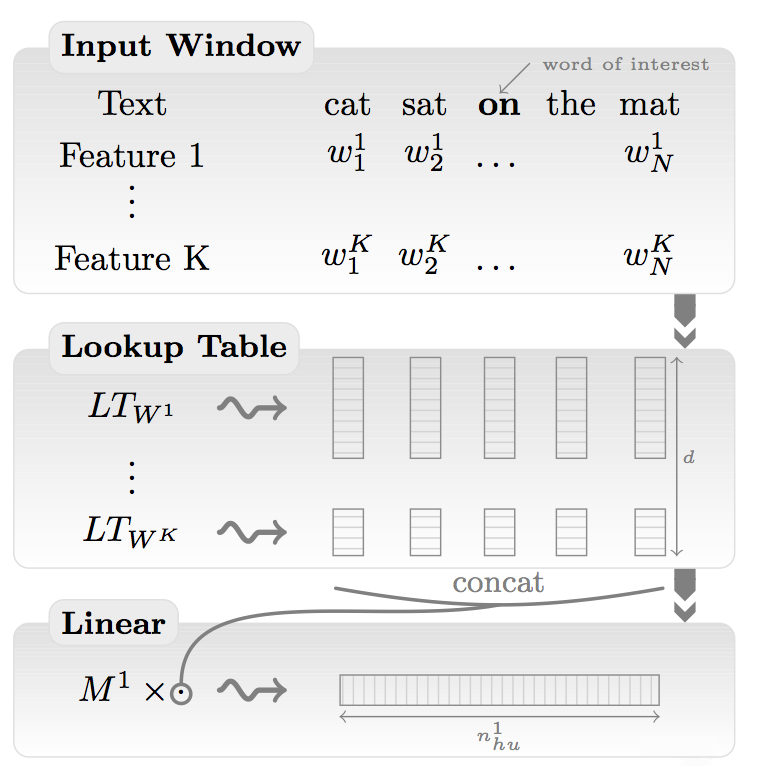
\includegraphics[scale=0.5]{../NLP-standalone-images/model.png}
\end{figure}

Because we have a small data set of annotated questions (see below), we used a linear model: a linear model has the advantage to have few parameters.
For example with a window approach of size 9 and words embedded in vectors of dimension 26,  this gives us $26\times 9\times 4 = 936$ parameters to learn.

In a first time we implemented our own linear classifier, but to improve the execution time, we finally used the \textit{LDA} classifier from the library scikit-learn. Few seconds of computation are now needed to train successfully the model.

\subsection{Data set}

Because we used supervised algorithms, we need a data set of annotated questions, in order to learn our model.
This data set was mostly built manually, because we did not find on the internet a data set that directly answering the problem of triple extraction.
Build this data set is a fastidious work. Currently our data set is composed of 300 questions.
We also wrote a script that generate keywords questions. This script gives us 500 keywords questions and make the module specialized on keywords questions.

We now denote $\mathcal{D}_{GC}$ (for \textit{Data set Grammatically Correct}) the data set of grammatically correct questions, $\mathcal{D}_{kw}$ for the data set of generated keywords questions and $\mathcal{D}_A = \mathcal{D}_{GC} \cup  \mathcal{D}_{KW}$ the complete data set.

\subsection{Results}

In this basic configuration, we can measure the accuracy of our algorithm, defined as the ratio of correctly classified words, for a specified data set.

Our methodology is the following: for a specified data set $\mathcal{D} \in \{\mathcal{D}_A, \mathcal{D}_{GC}, \mathcal{D}_{KW}\}$ we split $\mathcal{D}$ in two parts: the training set and the test set (90% of the data is for the training set and 10% for the testing set). We learn our classifier with the training set and then evaluate it on the test set.

\textbf{Remark}: to compute the accuracy of one variant of our algorithm we split the data set into testing and training set randomly, and we restart an experience 50 times. This make us sure of the precision of the estimated accuracy.

\begin{center}
\begin{tabular}{|l|c|r|}
  \hline
  Data set &  Testing accuracy  & Training accuracy \\
  \hline
  $\mathcal{D}_{GC}$ &  $75\%$& $81\%$  \\
  $\mathcal{D}_{KW}$ & $98\%$ & $98.3\%$ \\
  $\mathcal{D}_{A}$    & $83\%$ & $86\%$ \\
  \hline
\end{tabular}
\end{center}

We can conclude that this version of the algorithm is excellent for keyword questions, and not really good for grammatically correct questions.

\subsubsection{Bias vs Variance test}

We can plot the \textit{Bias versus Variance} curves:

\begin{figure}[!ht]
  \centering
  \caption{Bias vs Variance curve for the data set  $\mathcal{D}_{GC}$}
  \label{sandalone:bias_vs_variance_1}
    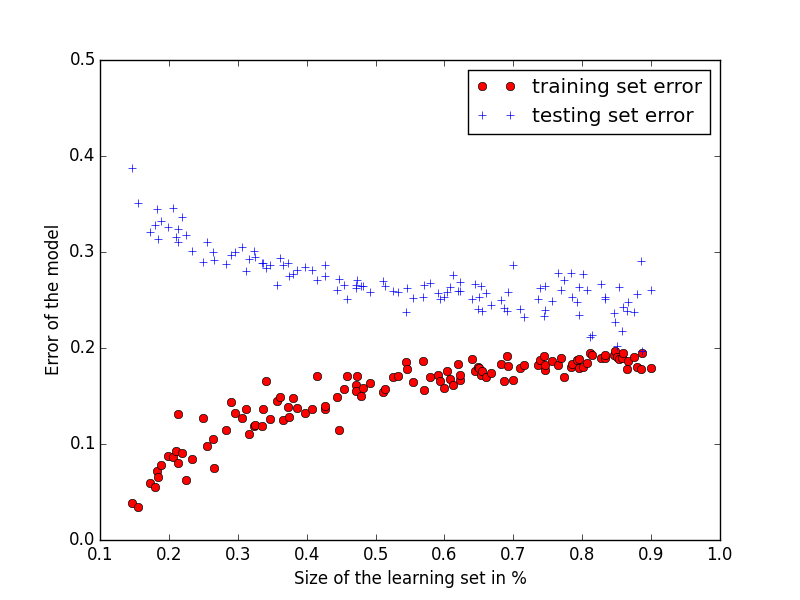
\includegraphics[scale=0.5]{../NLP-standalone-images/BiasVsVarianceD_GC.png}
\end{figure}

\begin{figure}[!ht]
  \centering
  \caption{Bias vs Variance curve for the data set  $\mathcal{D}_{KW}$}
  \label{sandalone:bias_vs_variance_2}
    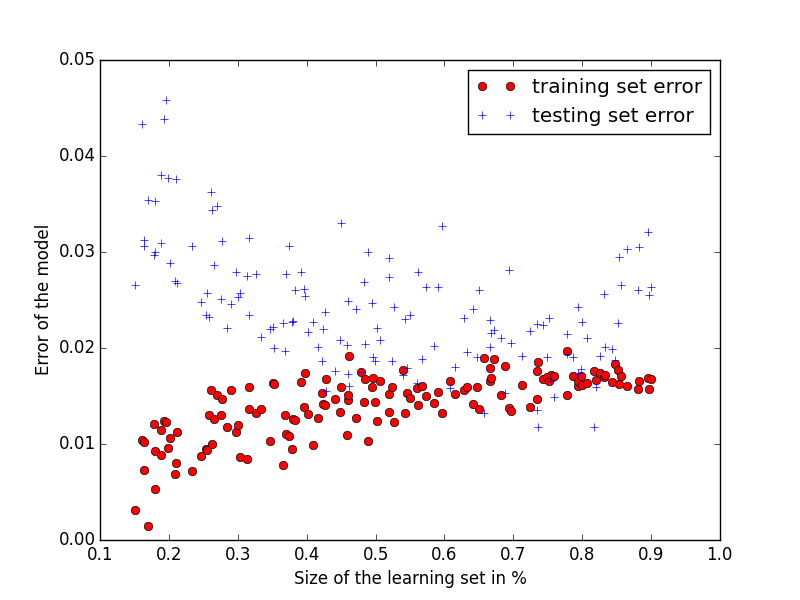
\includegraphics[scale=0.5]{../NLP-standalone-images/BiasVsVarianceD_KW.png}
\end{figure}

\begin{figure}[!ht]
  \centering
  \caption{Bias vs Variance curve for the data set  $\mathcal{D}_{A}$ }
  \label{sandalone:bias_vs_variance_3}
    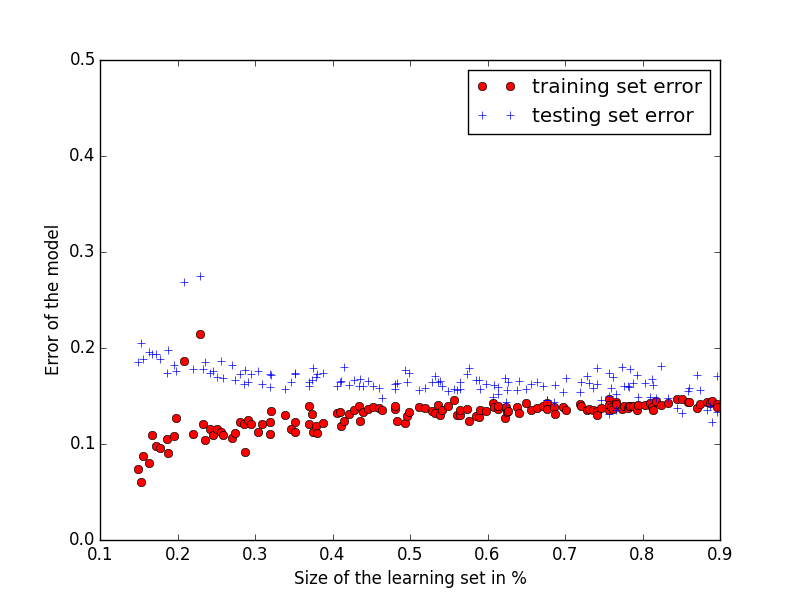
\includegraphics[scale=0.5]{../NLP-standalone-images/BiasVsVarianceD_A.png}
\end{figure}

These curves show us that there is a small gap between the two performances curves for the data set $\mathcal{D}_{GC}$: the data set of grammatically correct questions is too small to learn correctly the model.

However, when we add the keyword questions, the gap disappears: the model is learned correctly and the performances are good.

\subsection{Improvements of the algorithm}

\subsubsection{POS TAG features}

In order to help the classifier, we added POS TAG features: each word of the sentence is tagged with a grammatical tag (VERB, NOUN, PRON, ADJ, ...)

We use the NLTK pos tagger to do that. With such a tag, a word is encoded as a vector of dimension $26+11 = 37$.

This new feature helps improve the accuracy of the algorithm of few percents:

\begin{center}
\begin{tabular}{|l|c|r|}
  \hline
  Data set & Testing accuracy  without POS TAG & Testing accuracy  with POS TAG \\
  \hline
  $\mathcal{D}_{GC}$ &  $75\%$& $77.2\%$  \\
  $\mathcal{D}_{KW}$ & $98\%$ & $98.9\%$ \\
  $\mathcal{D}_{A}$    & $83\%$ & $86\%$ \\
  \hline
\end{tabular}
\end{center}


\subsection{Conclusion}

The initial goal was to make a concurrent of the grammatical approach to transform English questions into the data model. Due to the limited amount of time, we did not succeed to improve sufficiently the accuracy of the classifier to make this approach as good as the grammatical approach.

We decided then to focus on keywords questions, which are very important for a framework of question answering. For this task, whith a good data set of annotated keywords questions, this algorithm is really efficient.



\chapter{Wikidata module}
    \Wikidata module is our main proof of concept module which aims to demonstrate the ability of our framework to allow the easy creation of huge modules able to answer to thousand of questions. This module tries to answer to general knowledge using the data stored in \href{http://www.wikidata.org}{\Wikidata}.

\Wikidata is a free knowledge base hosted by the \Wikimedia as a sister project of \Wikipedia. It aims to build a free, collaborative, multilingual structured database of general knowledge (for more information see \cite{42240}). It provides a very good set of API that allows to consume and query \Wikidata content easily. \Wikidata is built upon elements (called items) that are about a given subject. Each item has a label, a description and some aliases to describe it and statements that provides data about this subject.

The \Wikidata module has been written in PHP in order to rely on good libraries that allow to easily interact with the \Wikidata API. Some contributions to these libraries have been done to make them fit better with the module use case. This module works in tree steps:
\begin{enumerate}
    \item It maps \texttt{resource} nodes of the question tree into \Wikidata content: the subjects of \texttt{triple} nodes are mapped to \Wikidata items, predicates to \Wikidata properties and objects to the type of value that is the range of the \Wikidata property of the predicate. If more than one match are possible, a tree per possible match is output.
    \item It performs queries against \Wikidata content using the previously done mapping to reduce as much as possible trees. When we have a \texttt{triple} node where the object is missing the module gets the \Wikidata item of the subject, looks for values for the predicate property and replace the \texttt{triple} node with a \texttt{resource} node for each value of the triple (and so builds as many trees as there are values). When there is a \texttt{triple} node with a missing subject the module uses the \href{http://wdq.wmflabs.org}{WikidataQuery} tool API with \href{https://github.com/ProjetPP/WikidataQueryApi}{a standalone wrapper} built for the project that returns all items with a given statement.
    \item It adds clean text representation of \texttt{resource} nodes added by the previous phase.
\end{enumerate}

The global architecture of the module has been quickly studied by one of the \Wikidata developers that found it fairly good.

    
\chapter{CAS module}
    \newcommand{\CalChAS}{\text{C}\hspace{-2pt}_{\text{AL}}\hspace{-3pt}\text{C}^{\text{H}}{\hspace{-4pt}}_\text{AS}}
\newcommand{\RR}{\mathbb{R}}
\newcommand{\CC}{\mathbb{C}}
\newcommand{\ZZ}{\mathbb{Z}}
\newcommand{\NN}{\mathbb{N}}
\newcommand{\dd}{\mathrm{d}}


\section{CAS}

A computer algebra system (CAS) module has been added to the PPP. Its work is to compute formally mathematical expressions.

\subsection{Input-output}

The CAS module takes as input a sentence whose string is a mathematical expression and output a resource of typed \texttt{math-latex} with two fields: one with a human readable formula and the other written in \LaTeX.

The difficulty is to decide whether a string represents a mathematical formula or not.

We use two tests. The first is a pre-treatment test. It checks whether the formula contains some substring which prove:
\begin{itemize}
    \item the formula is a mathematical expression, like "sqrt", "\textbackslash"\ldots,
    \item the formula is not a mathematical expression, like "who", "where", accented character\ldots.
\end{itemize}

But that does not eliminate all natural language questions, there still are false positive. Nevertheless, this test works in the larger part of cases.

\bigskip

So there is another test which is more precise. For example, a query like "author of bli-bla" will not be excluded by the previous algorithm. Moreover we see here why we can not consider '-' as a characteristic character of mathematical formula. The method is to verify if the module apply modifications.

In this example, the module has nothing to compute and just rearrange terms. So "author of bli-bla" becomes something like "author bli of - bla" considering 'author', 'bli', 'bla' and 'of' as variable. But we observe there was no modification. To do this test, the module counts each kind of symbol (except space and some particular symbols). If there is the same quantity of each symbol, we consider there is no modifications and the module decides he was useless and returns an empty list.

\subsection{Structure}

To do mathematical computations, we use a specific library: Sympy\footnote{\url{http://www.sympy.org/en/index.html}}. But this library is able to analyse only the input written with a syntax which is not intuitive and pretty complex.

To avoid arbitrary long computation, we launch Sympy evaluation in another process which has a limited memory and time.

To be usable, we define two parsers to handle other syntax: the syntax of Mathematica and another syntax we defined, which is designed to be intuitive and we named $\CalChAS$.

\subsection{Parsers}

\subsubsection{Mathematica parser}

This parser is quite simple. We use a LALR parser generated by PLY\footnote{\url{http://www.dabeaz.com/ply/}} (Python Lex Yacc). First, the input formula is parsed and transform into a tree, then, the tree is transform into a Sympy expression.

\subsubsection{\texorpdfstring{$\CalChAS$}{CalChAS} parser}

This syntax is more permissive. It allows arithmetic operations (division, multiplication, addition, subtraction, modulo, factorial, power) and several names for each standard function. For instance, the 
reciprocal of the hyperbolic sine can be written "argsh", "argsinh", "arcsh" etc.. So function names are matched with regular expression. For instance, the regex for the function argsinh is \begin{center}[\texttt{aA}](\texttt{r}([cg])?)?[\texttt{sS}](\texttt{in})?\texttt{h}\end{center}

The other feature we implement for flexibility is implicit multiplications. We understand "a b" as "a*b", "(a)b" as "(a)*b" and "(a)(b)" as "(a)*(b)". But "a(b)" have to remain unchanged because "a" can be a function so, "a(b)" is not "a*(b)".

This transformation is executed before the parser. The method is to launch the lexer a first time. Then we add the symbol "*" between the two symbols in one of these three configurations: ")("; a ")" and a identifier; two consecutive identifiers. Thus, we generate a modified formula with explicit multiplications and we can parse this expression.

The last feature implemented to make this syntax more permissive is to extend functions which are defined on a subset of $\RR$ like $\NN$. For example, the factorial which is defined on $\NN^*$ is extended on $\CC\setminus \ZZ^{-*}$ by using the function $\Gamma$. Thus, the expression $(-1/2)!$ has a meaning.

This syntax admits notation as defined in the standard ISO 31-11.

\subsection{Future work}

A parser for \LaTeX \ expressions can be implemented. We started to write a \LaTeX \ parser but it was more complicated than expected and actually it does not work for big operators like sum, product or integral.

We can also cover other mathematical fields. For instance:
\begin{itemize}
    \item probability,
    \item statistics,
    \item regression analysis,
    \item logic and set theory,
    \item discrete mathematics,
    \item sequences,
    \item plots.
\end{itemize}

We can imagine a more lenient syntax for functions which need to bound a variable when there is no ambiguities. For instance, we plan to allow "int(sin(x),0,Pi)" for "int(sin(x),x,0,Pi)" because $x$ is the only variable in this expression. If we are able to determine the list of variables, there is easy to create a new variable. That allows to define functions like $(k,n)\mapsto \binom{n}{k}$ on a larger set using a limit.

An important missing feature is the resolution of differential equations. In fact the \texttt{dsolve} function of Sympy does not work on every ODE and does not handle initial conditions. If this feature is not implemented soon, we will use the \texttt{dsolve} function of Sympy without initial conditions and determine constants with the function \texttt{solve}.

The other feature to implement, is the interpretation of mathematical queries expressed in natural language. For example, "integrate sin x dx from x=0 to pi" instead of "integrate(sin(x),x,0,pi)".


\chapter{Spell checker}
    \section{Spell Checker}


\addcontentsline{toc}{chapter}{Conclusion}
\chapter*{Conclusion}
    \begin{frame}[fragile]
    \frametitle{Nested question}

Who is the wife of the president of the United States?
    \begin{tabular}{ll}
        \alert{WolframAlpha} & Barack Obama\\
        \alert{Platypus} & Michelle Obama\\
    \end{tabular}

    \medbreak

    What are the birth dates of the daughters of the wife of the president of the United States?
    \begin{tabular}{ll}
        \alert{WolframAlpha} & Barack Obama\\
        \alert{Platypus} & Saturday, July 4, 1998 \& Sunday, June 10, 2001\\
    \end{tabular}
\end{frame}

\begin{frame}[fragile]
    \frametitle{Conjunction}

Who is an actor in Titanic and Inception?
    \begin{tabular}{ll}
        \alert{WolframAlpha} & all the actors of the two movies\\
        \alert{Platypus} & Leonardo DiCaprio\\
    \end{tabular}
\end{frame}

\section{Future work}

\begin{frame}[fragile]
    \frametitle{Better database}

    ``How fast is the TGV?''

    ``How wide is a tennis court?''

    Not answered by \alert{Wikidata}.

    \medbreak

    $\rightarrow$ Improve Wikidata?

    $\rightarrow$ Use another database?
\end{frame}

\begin{frame}[fragile]
    \frametitle{Better question parsing}

    ``What is the date of birth of Isaac Newton?''

    ``In which band does Bono sing?''

    Not parsed correctly.

    \medbreak

    $\rightarrow$ Train the Stanford CoreNLP library?

    $\rightarrow$ Improve the algorithm of the Grammatical module?

    $\rightarrow$ Better datasets for the ML modules?
\end{frame}

\begin{frame}[fragile]
    \frametitle{New modules}
    \begin{table}
    \Large
    \centering
    \begin{tabular}{ccc}
        \textcolor{mLightBrown}{cooking recipes} & \textcolor{mDarkBrown}{HAL} & \textcolor{mMediumBrown}{meteo} \\
        \multicolumn{3}{c}{\textcolor{mDarkTeal}{programming language interpreter}} \\
        \textcolor{mMediumBrown}{cinema} & \textcolor{mDarkTeal}{music} & \textcolor{mLightBrown}{literature}\\
        \textcolor{mDarkBrown}{OEIS} & \textcolor{mLightBrown}{translation} & \textcolor{mDarkTeal}{chemistry}\\
        \multicolumn{3}{c}{\textcolor{mMediumBrown}{sport statistics and predictions}} \\
    \end{tabular}
    \end{table}
\end{frame}

\begin{frame}[fragile]
    \frametitle{Some facts} % to update just before the presentation
    \alert{23 repositories}

    \begin{tabular}{lll}
        6 & PHP & Wikidata libraries and module\\
        12 & Python & Other modules, core, and libraries\\
        1 & C++ & ML-Reformulation\\
        1 & Shell & Deployment scripts\\
        1 & \LaTeX & This presentation and the report\\
        1 & Markdown & The specification\\
        1 & HTML/CSS/Javascript & The Web User Interface\\
        1 & HTML/CSS & The project's website\\
    \end{tabular}

    \alert{1982 commits} (without the ``integration'' repository, which has an automatic commit every 12h)

    \alert{26k lines} of code (13k in PHP, 10k in Python)
\end{frame}

\newlength{\logosize}
\setlength{\logosize}{12pt}
\begin{frame}[fragile]
    \frametitle{Stay tuned}
    \alert{\url{http://projetpp.github.io/}}

    \begin{tabular}{ll}
        
\includegraphics[width=\logosize]{Twitter_logo_blue.png} & \href{https://twitter.com/ProjetPP}{https://twitter.com/ProjetPP}\\
        
\includegraphics[width=\logosize]{GitHub-Mark-32px.png} &  \href{https://github.com/ProjetPP}{https://github.com/ProjetPP}\\
        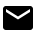
\includegraphics[width=\logosize]{ic_email_black_18dp.png} & \href{mailto:ppp@pony.ovh}{ppp@pony.ovh}\\
    \end{tabular}
\end{frame}


\begin{frame}
    \frametitle{Questions?}
    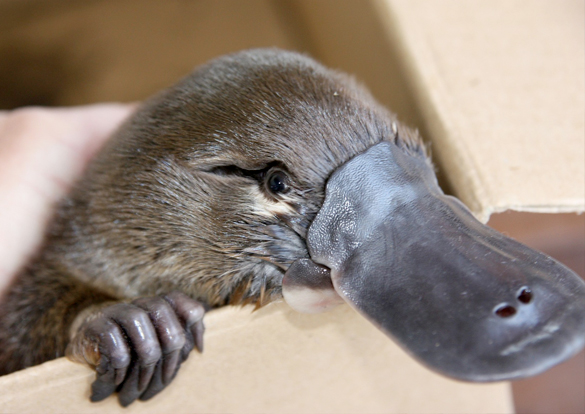
\includegraphics[width=\linewidth]{figures/platypusLg.jpg}
\end{frame}


\bibliographystyle{alpha}
\bibliography{bibliography}
\nocite{*}

\appendix

\chapter{Question parsing \--- Triples tree}

\begin{figure}[!ht]
\begin{verbatim}
{
    "type": "triple",
    "subject": {
        "type": "triple",
        "subject": {
            "type": "resource",
            "value": "United States"
        },
        "object": {
            "type": "missing"
        },
        "predicate": {
            "type": "resource",
            "value": "president"
        }
    },
    "object": {
        "type": "missing"
    },
    "predicate": {
        "type": "resource",
        "value": "birth place"
    }
}

\end{verbatim}

\caption{Triples tree produced by the question parsing grammatical module on \textit{Where was the president of the United States born?}}
\label{triple_tree}
\end{figure}

\chapter{Question parsing \--- Grammatical rules analysis}

\begin{figure}[!ht]
\begin{footnotesize}
\begin{verbatim}
    undef     : R0
    root      : R0
    dep       : R1
        aux       : remove
            auxpass   : remove
            cop       : impossible
        arg       : impossible
            agent     : R5
            comp      : R3
                acomp     : R3
                ccomp     : R5
                xcomp     : R3
                pcomp     : R3
                obj       : impossible
                    dobj      : R5
                    iobj      : R3
                    pobj      : R3
            subj      : impossible
                nsubj     : R2 (if the output node is a leaf) 
                            R5 otherwise
                    nsubjpass    : R5
                csubj     : impossible
                    csubjpass    : impossible
        cc        : impossible
        conj      : apply global transformation (conjunction) and produce Rconj
        expl      : remove
        mod       : R4
            amod      : merge (if the tag of the output node is neither ORDINAL nor JJS) 
                        otherwise apply global transformation and produce Rspl
            appos     : R4
            advcl     : R4
            det       : remove
            predet    : remove
            preconj   : remove
            vmod      : R3
            mwe       : merge
                mark      : remove
            advmod    : merge
                neg       : apply global transformation (conjunction) and produce Rconj
            rcmod     : R4
                quantmod  : remove
            nn        : merge
            npadvmod  : merge
                tmod      : R3
            num       : merge
            number    : merge
            prep      : R5
            prepc     : R5
            poss      : R5
            possessive: impossible
            prt       : merge
        parataxis : remove
        punct     : impossible
        ref       : impossible
        sdep      : impossible
            xsubj     : R3
        goeswith  : merge
        discourse : remove
\end{verbatim}
\end{footnotesize}
\caption{Replacement rules used by the question parsing grammatical module (\texttt{impossible} means that the relation is not supposed to happen, or is not supported yet by our algorithm)}
\label{gramm_rule}
\end{figure}

\chapter{Wikidata API examples}
\label{wikidata:api-examples}
\section{Retrieve entities}

Goal: get the item \texttt{Q42} (Douglas Adams).

Request: \url{http://www.wikidata.org/w/api.php?action=wbgetentities&ids=Q42&format=json&languages=en}

Partial response:
\begin{lstlisting}[language=json]
{
    "entities": {
        "Q42": {
            "id": "Q42",
            "type": "item",
            "aliases": {
                "en": [{"language": "en", "value": "Douglas Noel Adams"}]
            },
            "labels": {
                "en": {"language": "en",  "value": "Douglas Adams"}
            },
            "descriptions": {
                "en": {"language": "en", "value": "English writer and humorist"}
            },
            "claims": {
                "P31": [
                    {
                        "id": "Q42$F078E5B3-F9A8-480E-B7AC-D97778CBBEF9",
                        "mainsnak": {
                            "snaktype": "value",
                            "property": "P31",
                            "datatype": "wikibase-item",
                            "datavalue": {
                                "value": "Q5",
                                "type": "wikibase-entityid"
                            }
                        },
                        "type": "statement"
                    }
                ]
            },
            "sitelinks": {
                "enwiki": {"site": "enwiki", "title": "Douglas Adams"}
            }
        }
    }
}
\end{lstlisting}


\section{Retrieve entities}

Gloal: get items for the label "Douglas Adams".

Request: \url{http://www.wikidata.org/w/api.php?action=wbgetentities&ids=Q42&format=json&languages=en}

Partial response:
\begin{lstlisting}[language=json]
{
    "searchinfo":{"search": "Douglas Adams"},
    "search":[
        {
            "id": "Q42",
            "url": "//www.wikidata.org/wiki/Q42",
            "description": "English writer and humorist",
            "label": "Douglas Adams"
        }
    ]
}
\end{lstlisting}


\section{Do search with WikidataQuery}

Gloal: get items that have "position held" (P39) "president of the united States of America" (Q11696).

Documentation: \url{http://wdq.wmflabs.org/api_documentation.html}

Request: \url{http://wdq.wmflabs.org/api?q=CLAIM[39:11696]}

Partial response:
\begin{lstlisting}[language=json]
{
    "items": [23, 76, 91, 207]
}
\end{lstlisting}

\end{document}
